\documentclass[11pt,a4paper,draft=false]{report}
\usepackage{amsmath,amsthm,amssymb}
\usepackage{bm,txfonts}       % bm: bold for Greek letters, txfonts -> varmathbb
\usepackage{breqn}              % automatically brake line in equations
\usepackage{cancel}
\usepackage{siunitx}            % include before arydshln
\usepackage{arydshln}         % matrix dash lines
\usepackage{booktabs}         % tables
\usepackage{color,soul}         % used for \hl{}
\usepackage[inline]{enumitem}   % use to set labels in the enumerate environment
\usepackage{fullpage}
\usepackage[pdftex]{graphicx}
\graphicspath{{./figures/}{./tikz/}}
\DeclareGraphicsExtensions{.pdf,.png,.jpg}
\usepackage{caption}
\captionsetup{labelfont=bf}
\usepackage[caption=false,labelfont=bf]{subfig}
\usepackage{listings}
% \usepackage{algorithm}
% \usepackage{algorithmic}
\usepackage{url}
\usepackage[pdfpagelabels,pdfusetitle,colorlinks=true,pdfborder={0 0
  0},pdfauthor={Dimitar Stanev}]{hyperref}
\usepackage{natbib}
\bibliographystyle{IEEEtranN}

% indexing
%%%%%%%%%%%%%%%%%%%%%%%%%%%%%%%%%%%%%%%%%%%%%%%%%%%%%%%%%%%%%%%%%%%%%%%%%%%%%%%% 

% \usepackage{makeidx}
% \makeindex

% make use of \index{word} in text

% acronyms
%%%%%%%%%%%%%%%%%%%%%%%%%%%%%%%%%%%%%%%%%%%%%%%%%%%%%%%%%%%%%%%%%%%%%%%%%%%%%%%% 

\usepackage[acronym]{glossaries}

\newacronym{dofs}{DoFs}{Degrees of Freedom}
\newacronym{dof}{DoF}{Degree of Freedom}
\newacronym{eoms}{EoMs}{Equations of Motion}
\newacronym{fd}{FD}{Forward Dynamics}
\newacronym{pd}{PD}{Proportional Derivative}
\newacronym{cns}{CNS}{Central Nervous System}
\newacronym{lr}{LR}{Lateral Rectus}
\newacronym{sr}{SR}{Superior Rectus}
\newacronym{ir}{IR}{Inferior Rectus}
\newacronym{mr}{MR}{Medial Rectus}
\newacronym{so}{SO}{Superior Oblique}
\newacronym{io}{IO}{Inferior Oblique}
\newacronym{em}{EOMs}{Extraocular Muscles}
\newacronym{fl}{F-L}{Force-Length}
\newacronym{fv}{F-V}{Force-Velocity}
\newacronym{fpe}{F-PE}{Passive-Force-Length}
\newacronym{ft}{F-T}{Tendon-Force-Length}
\makeglossaries{}

% custom commands
%%%%%%%%%%%%%%%%%%%%%%%%%%%%%%%%%%%%%%%%%%%%%%%%%%%%%%%%%%%%%%%%%%%%%%%%%%%%%%%% 

\DeclareMathAlphabet\mathbfcal{OMS}{cmsy}{b}{n} % mathcal bf
\newcommand{\ten}[1]{\mathbfcal{#1}}
\newcommand{\mat}[1]{\bm{#1}}
\renewcommand*{\vec}[1]{\bm{#1}}
\newcommand{\R}[1]{\mathfrak{R}^{#1}}
\newcommand{\inr}[1]{\in\R{#1}}

\newcommand{\subfigureautorefname}{Figure} % subfloat
\renewcommand*{\figureautorefname}{Figure}
\renewcommand*{\sectionautorefname}{Section}
\renewcommand*{\subsectionautorefname}{Subsection}
\newcommand{\algorithmautorefname}{Algorithm}
\makeatletter
% \renewcommand\thealgorithm{\thechapter.\arabic{algorithm}}
\@addtoreset{algorithm}{chapter}
\makeatother
\def\equationautorefname~#1\null{Equation #1\null}

% in order to add newline in table cells
\usepackage{makecell}
\renewcommand\theadalign{bc}
\renewcommand\theadfont{\bfseries}
\renewcommand\theadgape{\Gape[4pt]}
\renewcommand\cellgape{\Gape[4pt]}

%%%%%%%%%%%%%%%%%%%%%%%%%%%%%%%%%%%%%%%%%%%%%%%%%%%%%%%%%%%%%%%%%%%%%%%%%%%%%%%% 
\title{An Open-Source OpenSim Oculomotor Model for Kinematics and Dynamics
  Simulation}

\author{Constantinos Filip, Dimitar Stanev\footnote{Electrical and Computer
    Engineering Department, University of Patras, Greece; Corresponding
    author: \url{stanev@ece.upatras.gr}}, and Konstantinos Moustakas}

\date{\today}

\begin{document}
%%%%%%%%%%%%%%%%%%%%%%%%%%%%%%%%%%%%%%%%%%%%%%%%%%%%%%%%%%%%%%%%%%%%%%%%%%%%%%%% 

\maketitle

%%%%%%%%%%%%%%%%%%%%%%%%%%%%%%%%%%%%%%%%%%%%%%%%%%%%%%%%%%%%%%%%%%%%%%%%%%%%%%%% 
\begin{abstract}
  Studying human eye movements has significant implications for improving our
  understanding of the oculomotor system and treating various visuomotor
  disorders. An open-source musculoskeletal model of the human eye, that can be
  used for kinematics and dynamics analysis, is constructed based on the data
  reported in literature and made publicly available\footnote{SimTK project:
    \url{https://simtk.org/projects/eye}}. The model is implemented in
  \texttt{OpenSim}, which is an open-source framework for modeling and
  simulation of musculoskeletal systems. The calibration of the model parameters
  is based on physiological measurements of the human eye. The model
  incorporates an eye globe, orbital suspension tissues and six extraocular
  muscles. The excitation and activation patterns for a variety of targets can
  be calculated using the proposed closed-loop fixation controller that drives
  the model to perform saccadic movements in a forward dynamics manner. The
  controller minimizes the error between the desired saccadic trajectory and the
  predicted movement. Consequently, this model enables the investigation muscle
  activation patterns during static fixation and analyze the dynamics of various
  eye movements.
\end{abstract}

%%%%%%%%%%%%%%%%%%%%%%%%%%%%%%%%%%%%%%%%%%%%%%%%%%%%%%%%%%%%%%%%%%%%%%%%%%%%%%%% 
\section*{Introduction}\label{sec:introduction}

Rapid and accurate eye movements are crucial for coordinated direction of
gaze~\cite{Lee2006}. Studying human eye movement has significant implications
for improving our understanding of the oculomotor system and treating visuomotor
disorders. Over the past decades, biomechanics simulation has provided the means
to analyze different human movements~\cite{Delp2007}. The same principles can be
used to analyze visual tasks by modeling the musculoskeletal properties of the
oculomotor system. Consequently, this model can be used to investigate muscle
activation patterns during static fixation, analyze the dynamics of various eye
movements, calculate metabolic costs and simulate eye disorders, such as
different forms of strabismus. Furthermore, it can be easily integrated with
available full body models in order to analyze the relation between the
vestibular and oculomotor systems.

Saccadic movements are a generated from a coordination of the six
\gls{em}. Clinical trials have provided a profound knowledge on the properties
of the \gls{em} and their line of action on the eye globe~\cite{Robinson1969a},
the resistive tension of the surrounding tissues~\cite{Collins1981} and the
length-tension relationship of the muscles~\cite{Iskander2018}. Various
computational models of the extraocular muscles and orbital mechanics have been
proposed, which provide insight and scientific bases for oculomotor
biomechanics, control of eye movement and binocular misalignment. These models
focus on the realism of muscle behavior and they were based on the viscoelastic
properties and physiological data \gls{em}.

The first 3D biomechanical model was developed by~\cite{Robinson1964a,
  Robinson1969}, who simplified the formulation by only considering the
elasticity of the \gls{em} ignoring their dynamics. The model incorporates
anatomically realistic muscle paths and empirical innervation-length-tension
relationships. To study the neural control of rapid saccadic movements, models
using anatomical and mechanical properties of \gls{em} have been developed by
accounting for the nonlinear muscle dynamics~\cite{Thelen2003a,
  Millard2013}. Such models, having the advantage of supporting dynamics
simulation, are used in conjunction with brain level
controllers~\cite{James2018}.

%%%%%%%%%%%%%%%%%%%%%%%%%%%%%%%%%%%%%%%%%%%%%%%%%%%%%%%%%%%%%%%%%%%%%%%%%%%%%%%% 
\section*{Methods}\label{sec:methods}

%%%%%%%%%%%%%%%%%%%%%%%%%%%%%%%%%%%%%%%%%%%%%%%%%%%%%%%%%%%%%%%%%%%%%%%%%%%%%%%% 
\subsection*{Eye Modeling}\label{sec:eye-Modeling}

The eye model consists of the eyeball, three pairs of \gls{em} and the
connective passive tissues. The size of an emmetropic human adult eye is
approximately $0.0242 \si{\m}$ (transverse, horizontal), $0.0237 \si{\m}$
(sagittal, vertical), $0.022 - 0.0248 \si{\m}$ (axial, anteroposterior) with no
significant difference between sexes and age groups. In the transverse diameter,
the eyeball size may vary from $0.021 \si{\m}$ to $0.027 \si{\m}$, thus it can
be approximated by a solid sphere of radius $r = 0.012 \si{\m}$. The eyeball was
constructed in \texttt{Blender}, using a spherical mesh with 32 segments and 12
rings, to construct the vitreous humor (body) as solid sphere and a conical
plate to construct the cornea.The weight of an average human eye is
$m = 0.0075 \si{\kg}$ and the moment of inertia can be calculated assuming a
spherical homogeneous and isotropic model $I = 2 / 5 m r^2$. The eye has three
rotational \gls{dofs} with respect to the frame of reference, namely
incyclotosion-excyclotosion ($x$-axis), adduction-abduction ($y$-axis) and
supraduction-infraduction ($z$-axis).

%%%%%%%%%%%%%%%%%%%%%%%%%%%%%%%%%%%%%%%%%%%%%%%%%%%%%%%%%%%%%%%%%%%%%%%%%%%%%%%% 
\subsection*{Muscle Modeling}\label{sec:muscle-modeling}

The six \gls{em}, including four rectus muscles and two oblique muscles, are
controlled by the cranial nerves so as to track a visual target and to stabilize
the image of the object. The \gls{lr} and \gls{mr} muscles form an antagonistic
pair that produce horizontal eye movements. The \gls{sr} and \gls{ir} muscles
form the vertical antagonist pair, which mainly controls vertical eye movement
and also affects rotation about the horizontal plane and the line of sight
(secondary action) due to insertion positions. The \gls{so} muscle passes
through the cartilaginous trochlea attached to the orbital wall, which reflects
the \gls{so} path by 51 deg. The \gls{io} muscle originates from the orbital
wall anteroinferior to the globe center and inserts on the sclera posterior to
the globe equator. The primary actions of \gls{so} and \gls{io} cause rotation
of the globe around the visual axis and vertical movement.

The model relies on the passive pulley assumption. \autoref{tab:muscle-path}
shows the positions of the origin, insertion and passive muscle pulleys for the
\gls{em}, defined in the local body coordinates of the eyeball. The data are
based on physiological measurements~\cite{Iskander2018}, with some minor
modification so as to prevent unrealistic muscle-surface penetration. Since no
position was documented for the origin of the \gls{so}, a point close to the
origins of the rectus muscles was chosen to match the fiber length in the
primary position of the \gls{so} muscle.

\begin{table}[ht]
  \centering
  \caption{Muscle path points for the six \gls{em} defined in the local frame of
    the eyeball (dimensions are given in meters).}\label{tab:muscle-path}
  \begin{tabular}{@{}cccccccccc@{}}
    \toprule
    \textbf{Muscle}
    & \multicolumn{3}{c}{\textbf{Origin}}
    & \multicolumn{3}{c}{\textbf{Pulley}}
    & \multicolumn{3}{c}{\textbf{Insertion}} \\
    \midrule
    & \textit{\textbf{Ox}} & \textit{\textbf{Oy}} & \textit{\textbf{Oz}}
    & \textit{\textbf{Px}} & \textit{\textbf{Py}} & \textit{\textbf{Pz}}
    & \textit{\textbf{Ix}} & \textit{\textbf{Iy}} & \textit{\textbf{Iz}} \\
    \midrule
    \gls{lr} & -0.034 & 0.0006 & -0.013 & -0.0102 & 0.0003 & 0.012 & 0.0065 & 0 & 0.0101 \\
    \gls{mr} & -0.030 & 0.0006 & -0.017 & -0.0053 & 0.00014 & -0.0146 & 0.0088 & 0 & -0.0096 \\
    \gls{sr} & -0.0317 & 0.0036 & -0.016 & -0.0092 & 0.012 & -0.002 & 0.0076 & 0.0104 & 0 \\
    \gls{ir} & -0.0317 & -0.0024 & -0.016 & -0.0042 & -0.0128 & -0.0042 & 0.00805 & -0.0102 & 0 \\
    \gls{so} & 0.0082 & 0.0122 & -0.0152 & -0.030834 & 0.001145 & -0.01644 & 0.0044 & 0.011 & 0.0029 \\
    \gls{io} & 0.0113 & -0.0154 & -0.0111 & -0.00718 & -0.0135 & 0 & -0.008 & 0 & 0.009 \\
    \bottomrule
  \end{tabular}
\end{table}

The Millard muscle model~\cite{Millard2013} has been adopted for the modeling of
the \gls{em}, permitting parameterization of the characteristic curves according
to the experimental measured data. The muscles were modeled using the rigid
tendon assumption that ignores the elasticity of the tendon. This means that the
series element of the muscle model is not included (the tendon length $l^T$ is
equal to the tendon slack length $l_s^T$). \gls{em} are considered
parallel-fibered muscles, so the pennation angle is zero ($\alpha = 0$). The
values for the maximum isometric force $f_o^M$, optimal fiber length $l_o^M$ and
tendon length $l^T$ are presented in~\autoref{tab:muscle-parameters}.

The \gls{fl} and \gls{fpe} characteristic curves of the \gls{em} differ
significantly from those of a skeletal muscle. As shown in
\autoref{fig:millard-curves}, we can fine-tune the curve parameters so as to fit
the experimental data available for the \gls{lr} muscle. The values for the
\gls{fl} and \gls{fpe} characteristic curves are summarized in
Tables~\ref{tab:fl-curve} and~\ref{tab:fpe-curve}, respectively. Due to lack of
data describing the other muscles, the parameters found for the \gls{lr} muscle
where used for the rest of the \gls{em}.

\begin{table}
  \centering
  \parbox{.45\linewidth}{
    \centering
    \caption{Parameters of the \gls{fl} characteristic curve for the
      \gls{em}.}\label{tab:fl-curve}
    \begin{tabular}{@{}cccccccccc@{}}
      \toprule
      \textbf{Parameter} & \textbf{Value} \\
      \midrule
      min norm active fiber length & 0.55 \\
      transition norm fiver length & 0.7 \\
      max norm active fiver length & 1.8 \\
      shallow ascending slope &  2.4 \\
      minimum value & 0.0 \\
      \bottomrule
    \end{tabular}
  }
  \quad
  \parbox{.45\linewidth}{
    \vspace{-1.5cm}
    \centering
    \caption{Parameters of the \gls{fpe} characteristic curve for the for the
      \gls{em}.}\label{tab:fpe-curve}
    \begin{tabular}{@{}cccccccccc@{}}
      \toprule
      \textbf{Parameter} & \textbf{Value} \\
      \midrule
      strain at zero force & -0.18 \\
      strain at one norm force & 0.4 \\
      \bottomrule
    \end{tabular}
  }
\end{table}

\begin{figure}[ht]
  \centering
  \subfloat[\gls{fl} curve]{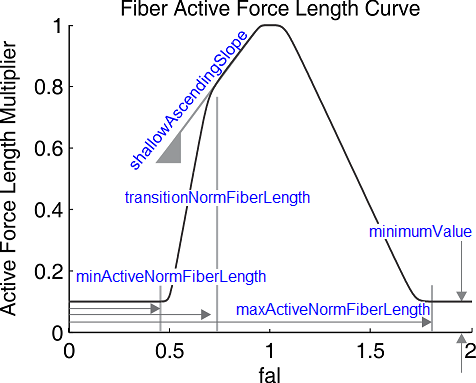
\includegraphics[width=0.5\textwidth,
    keepaspectratio]{active-force-length-curve.png}\label{fig:active-force-length-curve}}
  \subfloat[\gls{fl} curve]{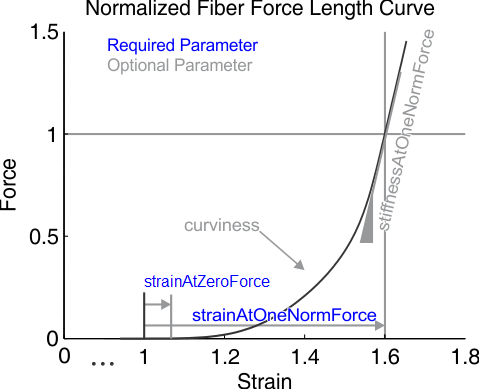
\includegraphics[width=0.5\textwidth,
    keepaspectratio]{passive-force-length-curve.png}\label{fig:passive-force-length-curve}}
  \caption{The \gls{fl} and \gls{fpe} curve definition for the Millard muscle
    model as implemented in \texttt{OpenSim}.}\label{fig:millard-curves}
\end{figure}

\gls{em} have a higher fraction of fast twitch fibers and thus different
\gls{fv} behavior, due to different structures compared to skeletal
muscles. Despite that, the default Millard \gls{fv} curve was used for the six
\gls{em}, since the behavior of the selected muscle model depends heavily on the
maximum contraction velocity $v^{\text{max}}$. The maximum muscle contraction
velocity is tuned so as to match the peak velocity of saccadic eye movement
$\omega^{\text{max}} = 15.7 \si{\radian / \second}$
($900 \si{\degree / \second}$). Following this definition, the maximum muscle
contraction velocity is given in optimal fiber length per seconds and it is thus
different for each \gls{em}, as their optimal fiber length is different
($v^{\text{max}} = \omega^{\text{max}} r / l_o^M$). Furthermore, since the optic
nerve is much shorter that the average muscle nerve, activation and deactivation
delays ($\tau_a = \tau_d = 5 \si{\milli\second}$) are smaller. Finally, two
separate wrapping spheres for the rectus muscles and the oblique muscles were
created, to avoid abnormal changes on the \gls{fl} curve as the eyeball rotates.

\begin{table}[ht]
  \centering
  \caption{Millard muscle parameters for the
    \gls{em}.}\label{tab:muscle-parameters}
  \begin{tabular}{@{}cccccccccc@{}}
    \toprule
    \thead{Muscle \\ \quad}
    & \thead{Maximum Isometric \\ Force (N)}  % math \si not in bold
    & \thead{Optimal Fiber \\ Length (m)}
    & \thead{Tendon Slack \\ Length (m)}
    & \thead{Maximum Contraction \\ Velocity (m / s)} \\
    \midrule
    \gls{lr} & 1.4710 & 0.04898 & 0.0084 & 3.8483 \\
    \gls{mr} & 1.5740 & 0.04084 & 0.0038 & 4.6155 \\
    \gls{sr} & 1.1768 & 0.04487 & 0.0054 & 4.2009 \\
    \gls{ir} & 1.4269 & 0.04549 & 0.0048 & 4.1437 \\
    \gls{so} & 0.6031 & 0.03956 & 0.0265 & 4.7648 \\
    \gls{io} & 0.5590 & 0.04110 & 0.0015 & 3.5863 \\
    \bottomrule
  \end{tabular}
\end{table}

%%%%%%%%%%%%%%%%%%%%%%%%%%%%%%%%%%%%%%%%%%%%%%%%%%%%%%%%%%%%%%%%%%%%%%%%%%%%%%%% 
\subsection*{Passive Connective Tissues}\label{sec:passive-connective-tissues}

The passive connective tissues apply a restoring force, which brings the eyeball
back to the central position when the net force from the \gls{em} is zero. These
tissues include all non-muscular suspensory tissues, such as Tenon's capsule,
the optic nerve, the fat pad and the conjunctiva. The force-displacement curve
of the net elasticity can be represented as

\begin{equation}\label{equ:passive-tissue}
  \vec{f}_t = -k_p \vec{q} - k_c 10^{-3} \vec{q}^3 - k_d * \vec{\dot{q}}
\end{equation}
%
where, $\vec{f}_t$ is the passive tissue forces,
$k_p= 0.002225 \si{\N \m / \radian}$, $k_c= 34.5297 \si{\N \m / \radian^3}$ and
$k_v= 0.002$ $\si{\N \m / (\radian / \s)}$ the constants and
$\vec{\dot{q}} \inr{3}$ the rotational coordinates of the
model~\cite{Collins1981} \hl{TODO}. These forces are modeled using
\texttt{OpenSim}'s expression based coordinate force.

% 0.33 * 9.8066500286389 * 10**-3 / (numpy.pi / 180) = 0.18542028707494282 * 0.012
% 1.56 * 9.8066500286389 * 10**-3 / (numpy.pi / 180) ** 3 = 2877.4856893811248 * 0.012

%%%%%%%%%%%%%%%%%%%%%%%%%%%%%%%%%%%%%%%%%%%%%%%%%%%%%%%%%%%%%%%%%%%%%%%%%%%%%%%% 
\section*{Results}\label{sec:results}

%%%%%%%%%%%%%%%%%%%%%%%%%%%%%%%%%%%%%%%%%%%%%%%%%%%%%%%%%%%%%%%%%%%%%%%%%%%%%%%% 
\subsection*{Fixation Controller}\label{sec:fixation-controller}

A fixation controller was implemented as a custom \texttt{OpenSim} plugin. The
parameters of the controller are: the desired horizontal $\theta_H$ and vertical
$\theta_V$ fixation angles (in degrees), the saccade onset and velocity (in
degrees), and the gains of \gls{pd} tracking controller ($k_p$, $k_d $). A
sigmoid function is used for generating smooth saccade trajectories

\begin{equation}\label{equ:sigmoid}
  \begin{aligned}
    \theta_d(t) &= \frac{a}{2} \Big(\tanh(b (t - t_0)) + 1\Big) \\
    \dot{\theta}_d(t) &= \frac{a b}{2} \Big(\tanh^2(b (t - t_0)) - 1\Big)
  \end{aligned}
\end{equation}
% 
where $\theta_d(t)$ and $\dot{\theta}_d(t)$ represent the desired orientation
and velocity at time $t$, $a$ the magnitude of the trajectory, $b$ the slope and
$t_0$ a time shift constant. Provided a fixation goal $\theta_g$, a desired
saccade velocity $\dot{\theta}_g$ and a saccade onset $t_g$ the parameters of
the sigmoid function are defined as follows $a = \theta_g$,
$b = 2 \dot{\theta}_g / \theta_g$ and $t_0 = t_s$. The \gls{pd} tracking
controller has the following form

\begin{equation}\label{equ:pd-controller}
  \ddot{\theta}(t) = k_p (\theta_d(t) - \theta(t)) + k_d (\dot{\theta}_d(t) -
  \dot{\theta}(t)).
\end{equation}

The sign and magnitude of $\ddot{\theta}(t)$ both for the horizontal and
vertical displacement of the fixation target is used to actuate the
corresponding muscles in order to achieve the desired goal. \autoref{fig:model}
presents an instance of the model during simulation with the corresponding
muscles activated. \autoref{fig:simulated-saccade} depicts the simulated
coordinates, speeds and estimated \gls{em} activations that reproduce the
desired saccade trajectory.

\begin{figure}[ht]
  \centering
  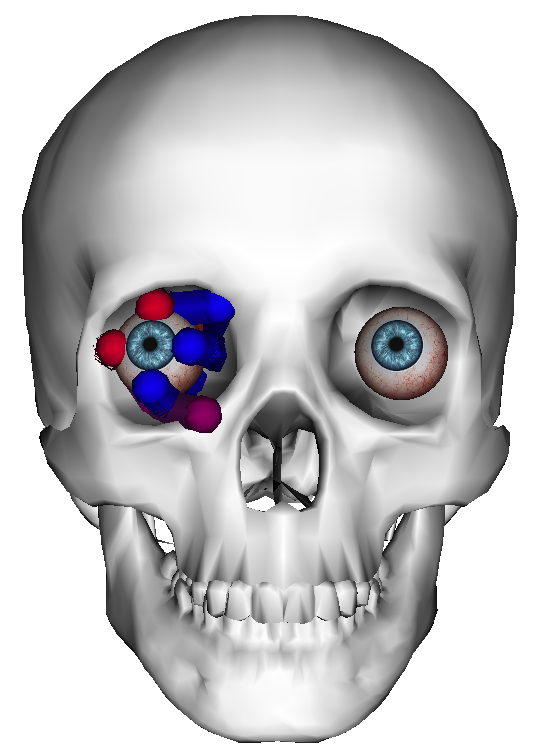
\includegraphics[width=.6\textwidth]{eye-model.png}
  \caption{Model with a fixation at $\theta_H = -15$ deg $\theta_V = 15$ deg
    during simulation. Blue denotes low and red high muscle activation
    levels.}\label{fig:model}
\end{figure}

\begin{figure}[ht]
  \centering
  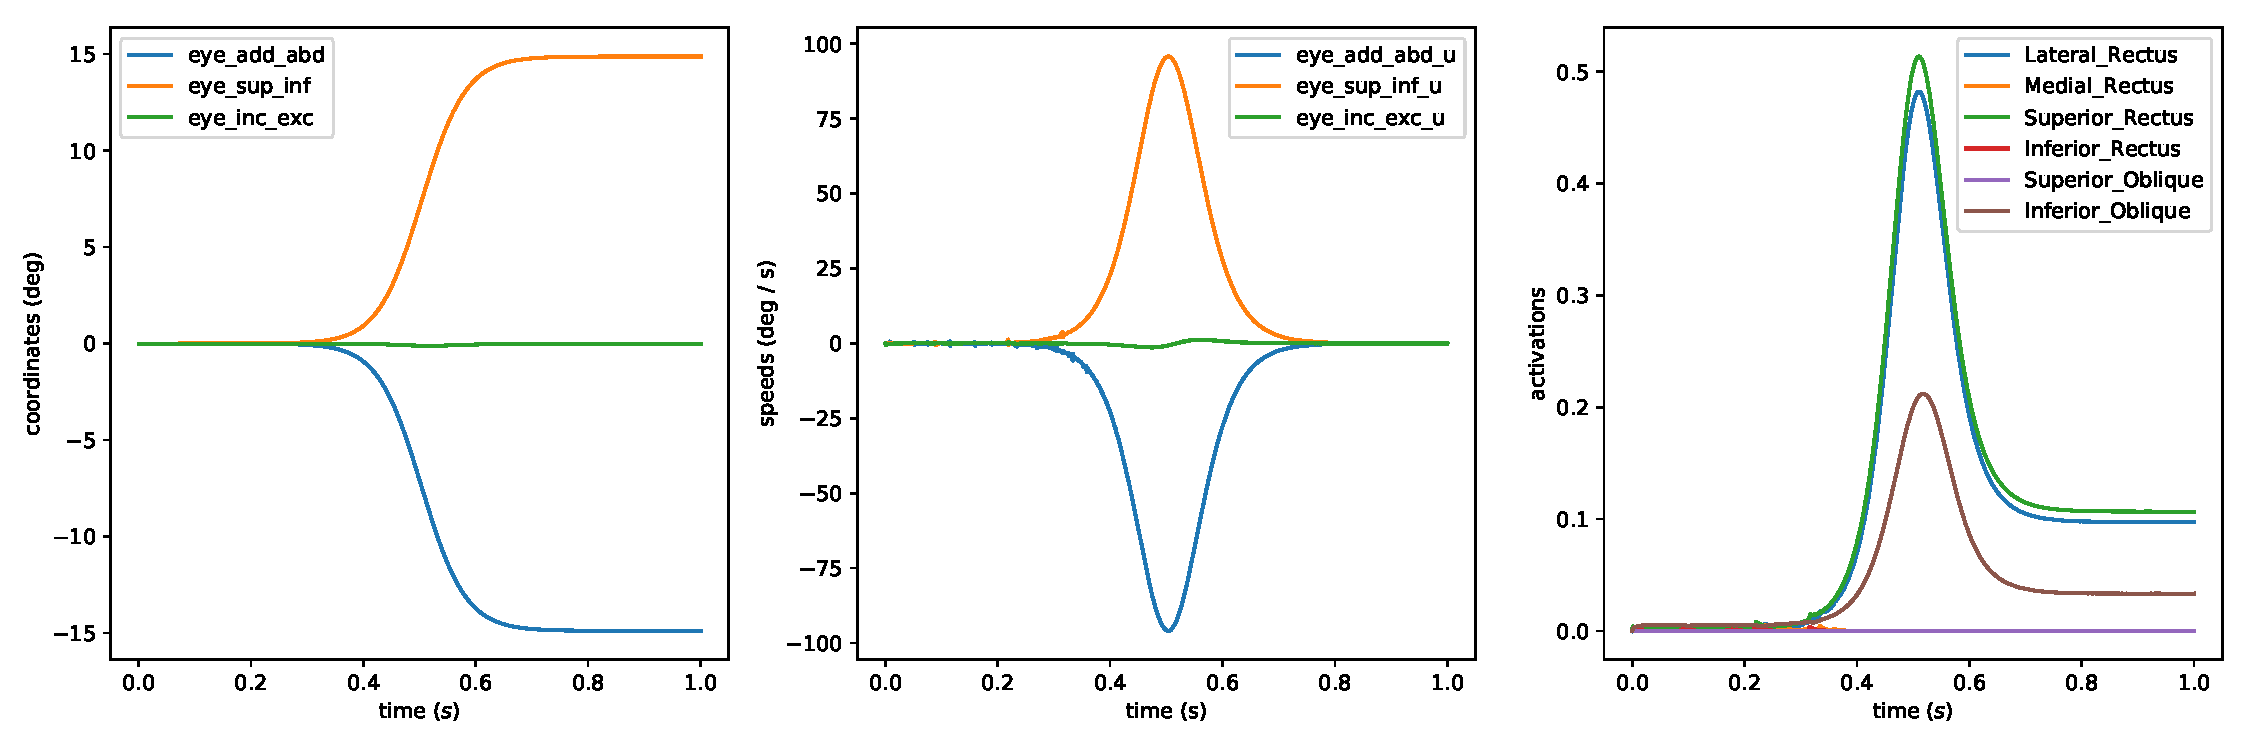
\includegraphics[width=1.\textwidth]{UPAT_Eye_Model_Passive_Pulleys_v3_States[-15][15].pdf}
  \caption{Simulated saccade response with a fixation at $\theta_H = -15$ deg
    $\theta_V = 15$ deg. The left subplot represents the simulated generalized
    coordinates; the middle the coordinate speeds; right the estimated \gls{em}
    activations.}\label{fig:simulated-saccade}
\end{figure}

%%%%%%%%%%%%%%%%%%%%%%%%%%%%%%%%%%%%%%%%%%%%%%%%%%%%%%%%%%%%%%%%%%%%%%%%%%%%%%%% 
\section*{Conclusion}\label{sec:concluison}

A realistic oculomotor model representing the motility of a normal human eye was
presented and made publicly available. The parameters of the model were
calibrated using available experimental measured data. The model can be used for
kinematics and dynamics analysis or as a tool for obtaining the muscle
activations that generate a desired saccade, using a closed-loop fixation
controller in a \gls{fd} manner. There is of course space for further
improvement, which will enhance the accuracy and the predictability of the
proposed computational model. In this study, we didn't attempt to model the
muscle pulleys~\cite{Kono2002a}, which vary as a function of the model
coordinates. Therefore, the users should consider performing further validation
of the eye model based on the requirements of the targeted utility and the
variables of interests.

%%%%%%%%%%%%%%%%%%%%%%%%%%%%%%%%%%%%%%%%%%%%%%%%%%%%%%%%%%%%%%%%%%%%%%%%%%%%%%%% 

\bibliography{mylibrary}
% \addcontentsline{toc}{chapter}{Bibliography}

%%%%%%%%%%%%%%%%%%%%%%%%%%%%%%%%%%%%%%%%%%%%%%%%%%%%%%%%%%%%%%%%%%%%%%%%%%%%%%%% 
\end{document}

%%% Local Variables:
%%% mode: latex
%%% TeX-master: t
%%% End:
